\chapter{Implementación de la solución}
\label{chapter:implementacion}

\section{Clases}

Para el desarrollo de la aplicación se usó el lenguaje Python, dividiendo la aplicación en clases que se pueden categorizar de la siguiente forma:

\subsection{Clases visuales}

\subsubsection{LatticeDesigner}
Esta es la clase principal de la aplicación, ya que es la encargada de iniciar el programa, cargando todas las dependencias necesarias para su ejecución, pero principalmente implementa la lógica de la parte visual del \emph{software}, es decir, de la creación y distribución en pantalla de los distintos elementos visuales, como ventanas, botones, campos de texto, etc., además de la interacción del usuario con estos. Cada reacción a una acción ejecutada sobre estos elementos es orquestada por esta clase.

\subsubsection{BitmapGrid}
La clase BitmapGrid es la encargada de manejar la grilla con la cuales los científicos diseñarán las configuraciones atómicas que se simularán. Para esto se basa en la biblioteca \emph{wx.grid} de \emph{wxPython}, una implementación de una planilla de cálculos tipo \emph{excel}, la cual es modificada para no poder ser editada y que las distintas acciones del \emph{mouse} sobre esta (click, seleccionar fila o columna, seleccionar un rango de celdas, etc.) generen cambios en el color de fondo de cada celda, pudiendo este ser negro o blanco, transformando esta planilla de cálculos en un mapa de bits binario.

Entre las características de este mapa de bits se encuentra la capacidad de crear figuras predefinidas rápidamente. Por ejemplo, se puede dibujar un cuadrilátero indicando el ancho, el alto y seleccionando la esquina superior derecha de esta figura. También es posible crear un círculo indicando el radio que tendrá este y su centro. Estas dos figuras predefinidas pueden combinarse para crear configuraciones más complejas, como un elipsoide, que son de mucha utilidad para los científicos (ver figura \ref{elipsoide}).

\begin{figure}[ht]
  \centering
  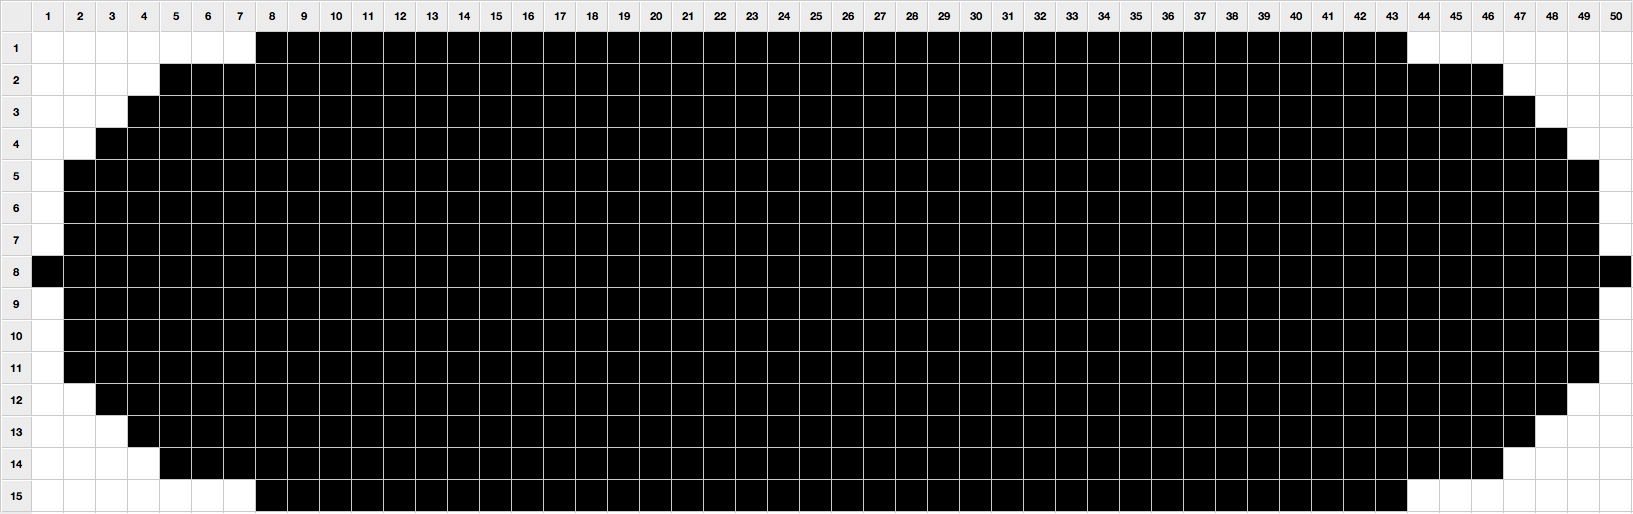
\includegraphics[scale=.25]{images/elipsoide}
  \caption{\em Mapa de bits binario con 2 figuras pre-diseñadas.}
  \label{elipsoide}
\end{figure}

\subsection{Clases 3D}

Estas clases son las encargadas de manejar los distintos \emph{canvas} que se usan en el \emph{software}, tanto para la visualización del diseño y del resultado de la simulación, como para ayudas referenciales para los científicos.

\subsubsection{AtomCanvas}

La clase AtomCanvas es la más importante con respecto a la visualización 3D, ya que es la encargada de mostrar en pantalla tanto el diseño de los objetos sobre los cuales se correrá la simulación como los resultados de estas usando OpenGL. En el desarrollo de esta clase se puso énfasis en la optimización, pudiendo mostrar sin mayores demoras más de 20.000 átomos. Para tener una idea un sistema promedio escalado analizado por los científicos usa 3.000 átomos (TODO: CONFIRMAR).

Otra de las tareas de esta clase es manejar las distintas interacciones del usuario, tanto con el teclado como con el \emph{mouse} con las representaciones en 3D, como rotaciones, movimientos y \emph{zoom}.

Para la visualización del diseño se usan esferas de distintos colores, representando cada uno de los distintos tipos de átomos que pueden haber según la estructura cúbica elegida. En las figuras \ref{atomCanvas-SC}, \ref{atomCanvas-BCC} y \ref{atomCanvas-FCC} se representan una estructura de 5x5 átomos, con 3 capas, siendo diferente solo la estructura cristalina elegida.

\begin{figure}[ht]
  \centering
  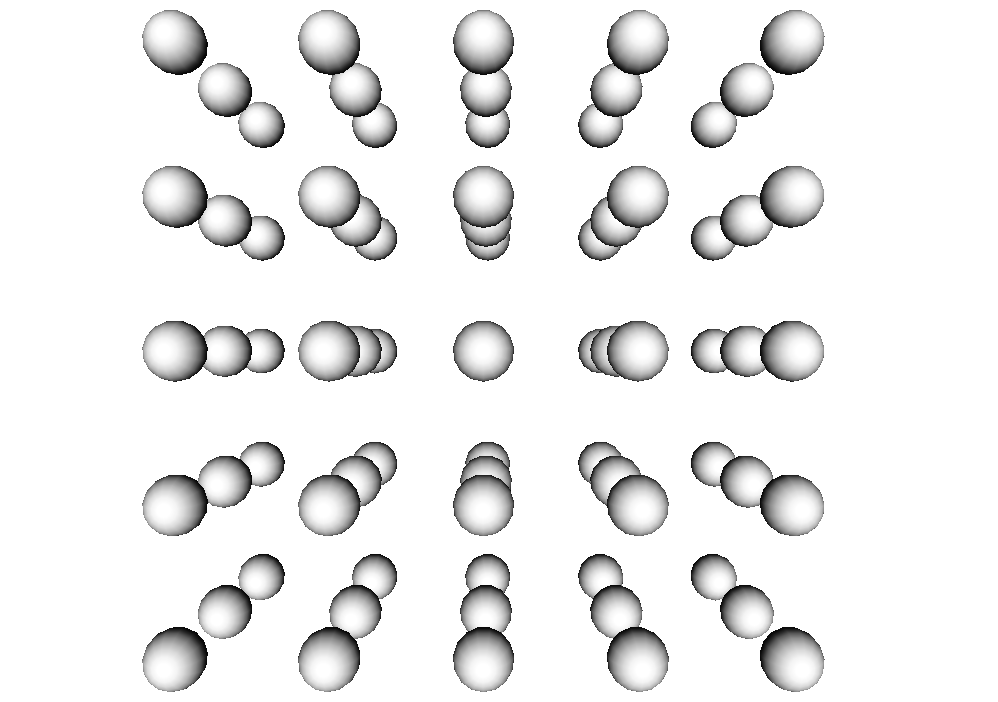
\includegraphics[scale=.3]{images/atomCanvas-SC}
  \caption{\em En un SC todos los átomos son blancos.}
  \label{atomCanvas-SC}
\end{figure}

\begin{figure}[ht]
  \centering
  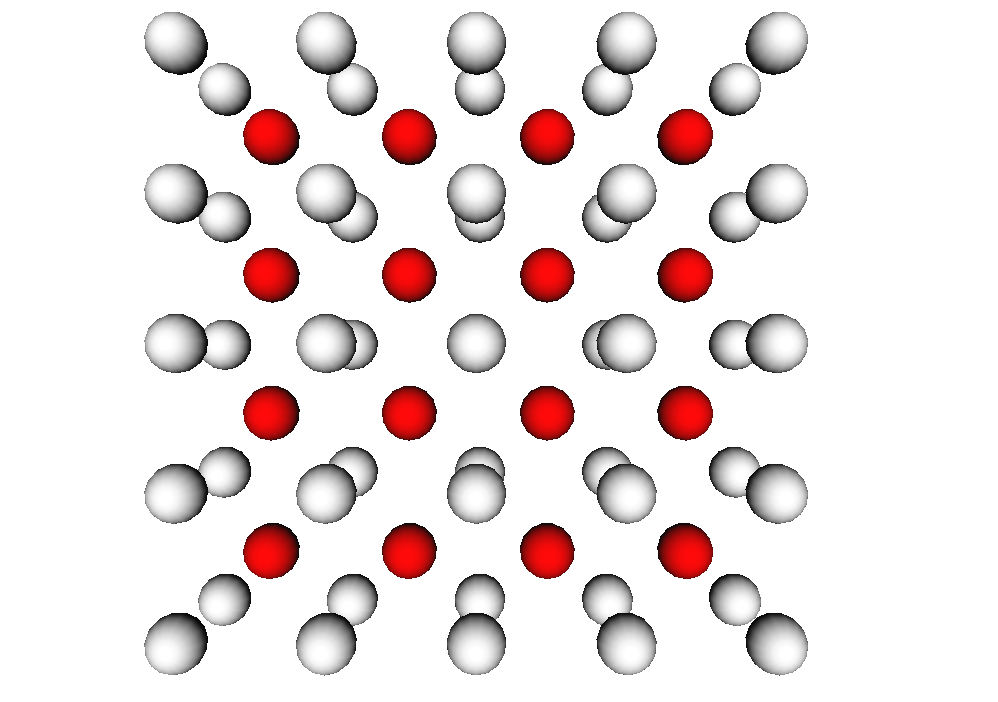
\includegraphics[scale=.3]{images/atomCanvas-BCC}
  \caption{\em En un BCC los átomos centrales son rojos.}
  \label{atomCanvas-BCC}
\end{figure}

\begin{figure}[ht]
  \centering
  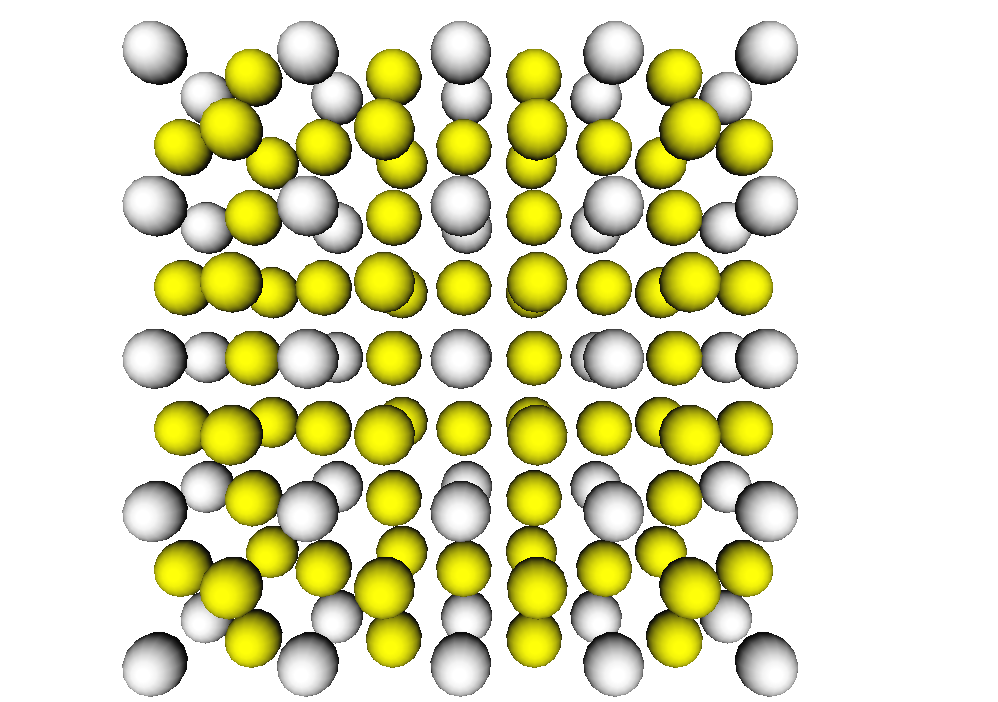
\includegraphics[scale=.35]{images/atomCanvas-FCC}
  \caption{\em En un FCC los átomos de las caras son amarillos.}
  \label{atomCanvas-FCC}
\end{figure}

En el caso de la visualización de resultados se usan flechas de colores como representación del momento magnético. Para asignar un color a una flecha se parte de la premisa que en tiempo t=0 el campo magnético externo está siendo aplicado hacia un eje, y por lo tanto inicialmente todos los vectores tendrán la misma magnitud, sentido y dirección, paralelos al campo externo, como se puede notar en la figura \ref{atomCanvas-vectores-inicial}. Además se sabe que en ese momento su magnitud es máxima. Si inicialmente todos los vectores son paralelos al eje A, se usa la componente â de cada vector para definir el color. Si la componente es 0 entonces será de color verde; si la magnitud es máxima en sentido contrario a los vectores iniciales el color será azul; si la magnitud es máxima en el mismo sentido de los vectores iniciales el color será rojo. Como se puede inferir la escala va desde azul a rojo, siendo este último color el inicial para todos los vectores. En la figura \ref{atomCanvas-vectores-colores} se puede ver los distintos colores según la componente $\hat{i}$ de los vectores, dado que el campo externo inicial tiene sentido $[1, 0, 0]$.

\begin{figure}[ht]
  \centering
  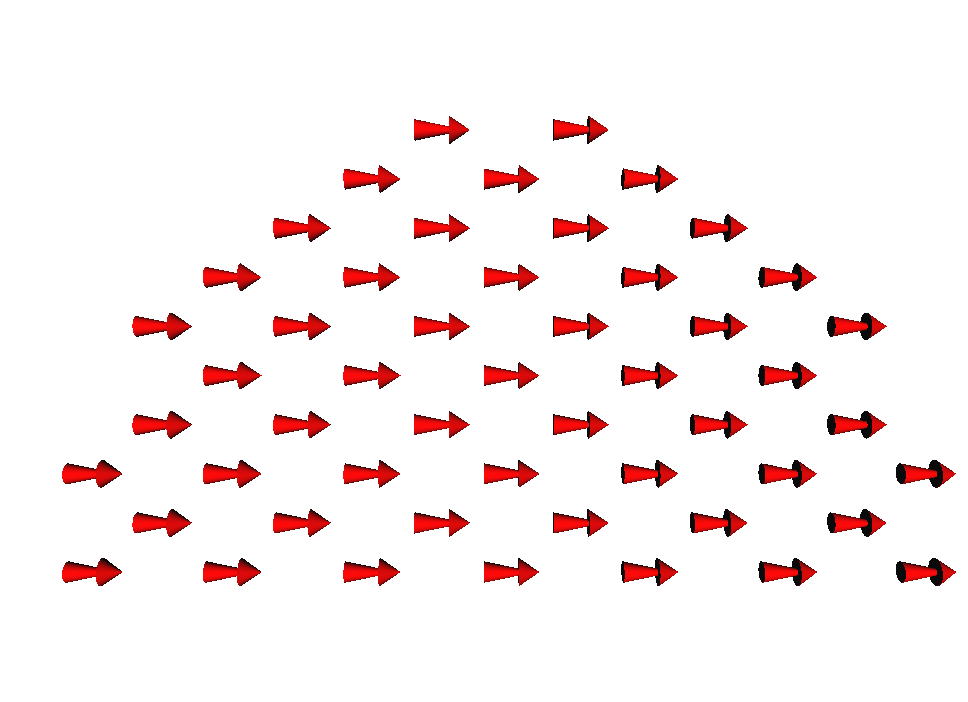
\includegraphics[scale=.3]{images/atomCanvas-vectores-inicial}
  \caption{\em Estado inicial de la visualización, con todos los vectores rojos paralelos al campo magnético externo inicial.}
  \label{atomCanvas-vectores-inicial}
\end{figure}

\begin{figure}[ht]
  \centering
  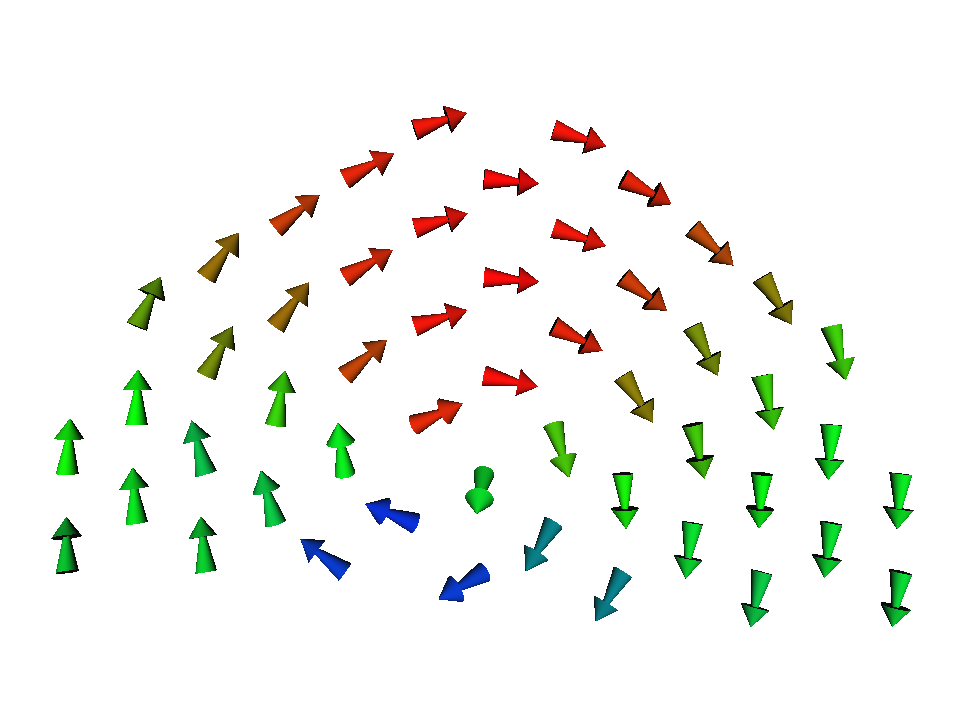
\includegraphics[scale=.3]{images/atomCanvas-vectores-colores}
  \caption{\em Vectores de distintos colores según la componente $\hat{i}$.}
  \label{atomCanvas-vectores-colores}
\end{figure}

\subsubsection{Axes}

La clase Axes es la encargada de mostrar los ejes coordenados de los distintos canvas, tanto del de diseño de objetos como el de visualización de resultados, usando Open GL.
Cada eje se representa con su propio color, usando azul, rojo y verde para los ejes X, Y y Z respectivamente, y una etiqueta con el mismo color, de forma de hacerlo fácil de visualizar para el usuario.
Debido al diseño del \emph{software}, donde las distintas funciones del programa (diseño y visualización) se seleccionan mediante pestañas, esta clase debe ser instanciada 2 veces, ya que no es posible usar la misma instancia en ambas secciones. Estas se comunican directamente con AtomCanvas para obtener los distintos parámetros de rotación de forma que los ejes sean coherentes a la imagen mostrada.

\begin{figure}[ht]
  \centering
  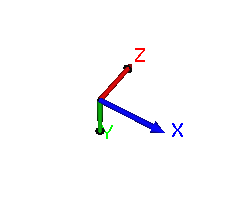
\includegraphics[scale=1]{images/axes}
  \caption{\em Representación visual de los ejes coordenados.}
\end{figure}

\subsection{Clases de cubos}


Las clases de cubos son 3 clases (\emph{SC}, \emph{BCC} y \emph{FCC}) que heredan de un mismo padre, \emph{Cube}. Estas crean los átomos de un objeto que se está diseñando. Las 3 clases hermanas tienen solo 2 métodos: \emph{calculate} y \emph{find\_neighborhood}. El primero se encarga de identificar todos los átomos que conforman la configuración atómica, dados los parámetros físicos como la estructura de la primera capa. El segundo define cuales son los parámetros para llamar al método \emph{find\_neighborhood} de la súper clase, el que busca todos los vecinos inmediatos para cada átomo. Estos parametros son necesarios para exportar el archivo que luego servirá de entrada para la simulación.

\subsubsection{Cube}
TBD


\subsubsection{SC}
SC es la clase que maneja los cubos simples (\emph{Simple Cubic} o \emph{SC}), estas estructuras cúbicas se caracterizan por tener un átomo en cada uno de sus vértices, por lo que la identificación de sus átomos se reduce a simplemente repetir la capa superior tantas veces como sea indicado en la entrada de propiedades físicas. Para encontrar el vecindario es necesario buscar todos los átomos que estén en las siguientes posiciones relativas [-1,0,0], [1,0,0], [0,-1,0], [0,1,0], [0,0,-1] y [0,0,1], por lo que el tamaño máximo de su vecindad es de 6 átomos.

\subsubsection{BCC}
BCC es la clase que maneja los cubos centrados en el cuerpo (\emph{Body Centered Cubic} o \emph{BCC}), que son las estructuras cúbicas que además de tener un átomo en cada vértice de los cubos tienen uno en el centro de cada uno de estos. Esto implica que en la identificación de átomos se debe trabajar con una capa intermedia que contiene los centros de cada cubo. por ejemplo, para una estructura de 5 capas quedaría así:
\begin{center}
  \begin{tabular}{ c | l }
    \# & Capa \\
    \hline
    1 & Primaria \\
    2 & Intermedia \\
    3 & Primaria \\
    4 & Intermedia \\
    5 & Primaria \\
    \hline
  \end{tabular}
\end{center}

La regla para agregar un átomo central es que debe tener un cubo de átomos a su alrededor, y en caso que el cubo no esté completo simplemente se usan las capas primarias, como se puede notar en las figuras \ref{BCC-incomplete-molecule} y \ref{BCC-complete-molecule}.

\begin{figure}[ht]
  \centering
  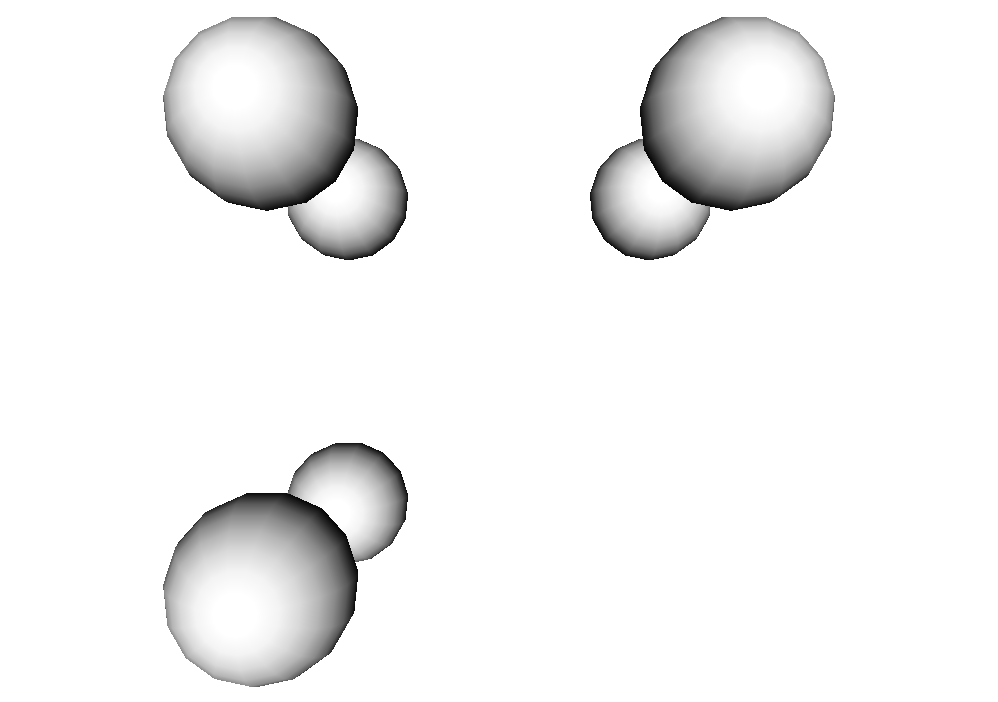
\includegraphics[scale=.3]{images/BCC-incomplete-molecule}
  \caption{\em Cubo BCC incompleto, sin átomo central}
  \label{BCC-incomplete-molecule}
\end{figure}

\begin{figure}[ht]
  \centering
  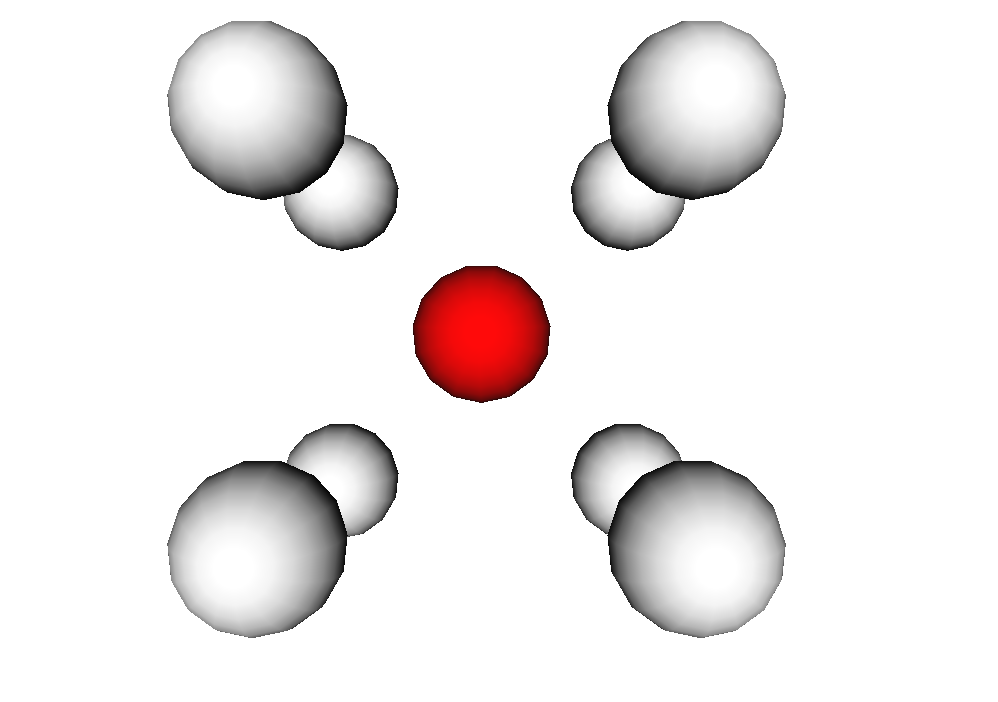
\includegraphics[scale=.3]{images/BCC-complete-molecule}
  \caption{\em Cubo BCC completo, con átomo central}
  \label{BCC-complete-molecule}
\end{figure}

En el caso de los BCC los átomos que conforman la vecindad siempre estarán en las posiciones relativas $[\pm 0.5, \pm 0.5, \pm 0.5]$, es decir, cada átomo puede tener una vecindad compuesta por hasta 8 átomos.

\subsubsection{FCC}
FCC es la clase que maneja los cubos centrados en las caras (\emph{Face Centered Cubic} o \emph{FCC}), los cuales se caracterizan por tener un átomo extra por cara además de uno en cada uno de sus vértices, por lo que además de tener que crear una capa intermedia es necesario modificar la capa primaria, es decir, la que crea el usuario usando el mapa de bits. La regla para agregar estos átomos en las caras es que ellos estén en la diagonal creada por otros 2 átomos, en cualquier dirección. En la figura \ref{FCC-diagonal} se ve como en una estructura cúbica de 1x2, como en una de sus caras se forma una diagonal entre 2 átomos y por lo tanto es necesario agregar un átomo extra en una capa intermedia.

\begin{figure}[ht]
  \centering
  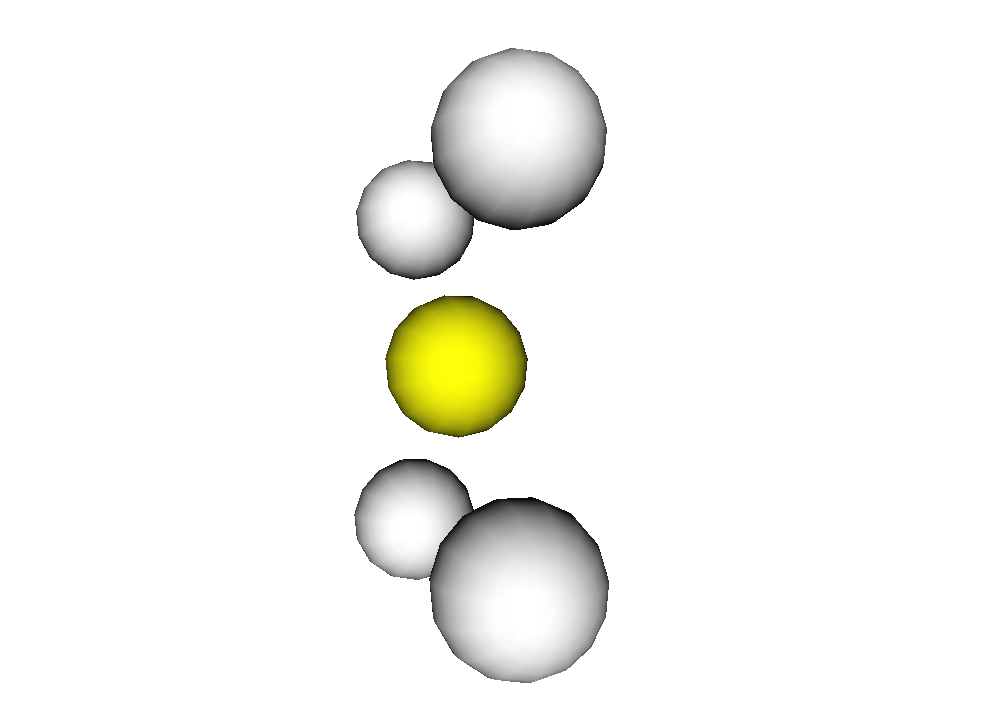
\includegraphics[scale=.3]{images/FCC-diagonal}
  \caption{\em Estructura cúbica FCC, con átomo en una de sus caras}
  \label{FCC-diagonal}
\end{figure}

La vecindad de estas estructuras cúbicas está dada por la posición relativa dada por $[\alpha, \beta, \gamma]$, donde:

\[
	\begin{cases}
		$$(\alpha = \pm 0.5; \beta = \pm 0.5; \gamma = 0)$$ \\
		$$(\alpha = \pm 0.5; \beta = 0; \gamma = \pm 0.5)$$ \\
		$$(\alpha = 0; \beta = \pm 0.5; \gamma = \pm 0.5)$$
	\end{cases}
\]
% 		$n/2 & \quad \text{if } n \text{ is even}\\ -(n+1)/2 & \quad \text{if } n \text{ is odd}\\ 

% $$  \vee  \vee $$

Lo que resulta en 12 posiciones posibles, siendo este el número máximo de átomos en una vecindad.